\chapter{绪论}
 % 简短的介绍

\section{研究背景及意义}
在中国改革开放和国际化进程的不断深入下,全社会对市场、对营销、对管理的态度发生了从无知到有知,从漠视到重视的巨大转变。时至今日,中国好像从来没有与世界的脉搏如此的接近过,同样,我们的企业和国家也从来没有如此深切地感受到全球化竞争是如此的残酷。因为市场竞争的不断加剧,每个企业都在努力寻找着自己的核心竞争能力,以期望能在激烈的商业竞争中取得优势。所以,这就给当前的商业研究提出了新的课题,直复营销(Direct Marketing)就是其中一个重要的研究方向。

直复营销是指企业通过媒介(如邮件、电话等)向目标市场成员发布营销信息,进而寻求对方直接回应(问询或订购)的营销模式\citep{王广宇2013客户关系管理},其简化过程如图$\ref{fig:直复营销示意图}$所示,如果按照营销时间是否具有周期性可以将直复营销分为定期直复营销和不定期直复营销。在直复营销场景中,营销人员首先需要根据客户的个人资料和历史响应记录(问询或订购)等信息,来构建客户的响应模型。然后,在每一次的营销活动前,再根据构建的响应模型来决定应该对哪些目标客户进行这一次的营销行为。通常情况下,为了使每次营销活动能够产生的利润最大化,营销人员只会选择那些可以使企业产生正向(非零)利润(收益减去成本)的客户进行营销。但是,在现实应用中,因为场景的复杂性往往很难获得一个高效而稳定的营销策略。

	\begin{figure}[htbp]
	\centering
	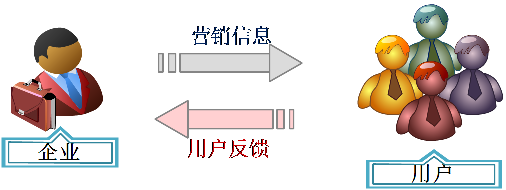
\includegraphics[width=0.65\textwidth]{直效营销示意图}
	\caption{直复营销简化示意图}
	\label{fig:直复营销示意图}
	\end{figure}

近年来,随着信息化和智能化的快速发展,机器学习技术正日益成为直复营销研究的重要方向。最开始,研究人员通过使用监督学习和非监督学习方法中的经典分类模型,以营销决策中的低错误率为学习目标,来解决上述问题。但是,在营销场景中,对不同客户的错误分类给企业所带来的损失是不同的,所以传统的分类算法具有很大的局限性。基于这个不足,研究人员后续提出了很多基于代价敏感(Cost-sensitive)的学习方法,这些方法将不同样本的错误分类赋予不同的惩罚代价,因而当应用于直复营销场景时,可以取得比传统分类算法更好的效果。

但是,在使用上述基于监督学习和非监督学习的方法时,只能最大化单次决策的即时收益,即前一个决策和后一个决策之间是独立的。而在像直复营销这类应用场景中,随着时间的推移需要不断地做出决策,属于序贯决策问题,所以,当营销人员在进行营销决策时,不仅需要考虑到单次营销的成本和收益,还要考虑到随着时间的推移,该次营销对后续营销结果可能产生的影响。比如:在某一次的营销活动中,企业从某个客户那么所得到的预期收益可能会大于营销成本(即利润为负),但是,这次的营销也可能会使得该客户在之后的营销活动中产生更多的消费(即企业获得更多的收益)。所以,在某些时刻,为了让客户在连续的营销活动中能产生更多的利润,营销人员可能要牺牲短期的利润,以达到最大化客户生命周期价值的目的。而基于监督学习或者非监督学习的算法很难实现这一点。

强化学习(Reinforcement Learning, RL)主要用于解决序贯决策问题,它是机器学习的重要组成部分,其学习过程如图$\ref{fig:强化学习过程}$所示:通过智能体(Agent)不断地与环境(environment)进行交互,并从环境反馈的延迟奖赏中学习状态与行为之间的映射关系,以使得可以达到累积奖赏最大化\citep{2016面向强化学习的模型学习算法研究}。从以上交互过程中,可以发现:强化学习在学习过程中考虑到了延迟回报,并且只关心当前采取什么行为可以使整个任务序列达到累积奖赏最大化,因此,强化学习算法可以很好地解决直复营销场景中营销决策点间的相互影响问题,进而实现最大化客户生命周期价值的目标,这也是本文选择使用强化学习技术解决直复营销问题的出发点。特别地,本文只关注基于值函数的强化学习方法。

\begin{figure}[htbp]
\centering
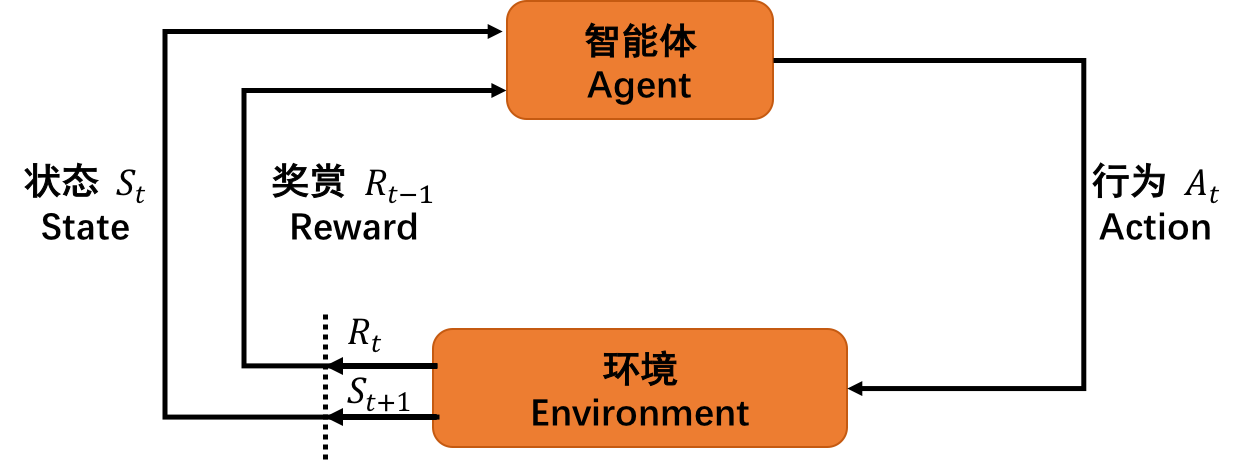
\includegraphics[width=0.8\textwidth]{强化学习过程_}
\caption{强化学习的交互过程}
\label{fig:强化学习过程}
\end{figure}

强化学习是从控制学、心理学、统计学和运筹学等重多学科交叉发展而来的。在1980年到2000年之间,经过众多学者的不懈努力,强化学习的理论研究取得了重大进展,随后被越来越多地用于工业控制、作业调度和机器学习等领域。比如,Macek等人将强化学习技术应用于机器人躲避障碍物\citep{macek2002reinforcement},Tesaruo等人结合神经网络将强化学习应用于西洋双陆棋中\citep{tesauro2006hybrid}。2016年和2017年,DeepMind团队利用深度强化学习(Deep Reinforcement Learning, DRL)技术研发的智能围棋程序AlphaGo大胜世界冠军李世石和柯洁,并引发了研究强化学习的热潮。

虽然强化学习在一些的实际应用中已经取得了重大进展,但是由于强化学习算法理论的复杂性,加之不同应用场景的特殊性,使得强化学习在实际应用中仍然面临着许多困难。在直复营销场景中,虽然近年来已经有学者开始使用强化学习技术来解决直复营销的决策问题,但是以下问题仍然没有得到有效的解决:

(a)在不定期直复营销场景中,因为营销决策点间的时间间隔是不固定的,所以这就会改变回报的计算方式,从而给奖赏带来了一定的噪声影响,进而会影响值函数的学习和优化。

(b)在实际应用中,随着数据量的提升,传统强化学习方法容易出现训练速度慢、学习效率不高的问题。

(c)在直复营销场景中,因为客户的状态存在部分可观测(Partial Observability)问题,所以为了更好地定义客户的状态以进行更高效的策略学习,在实际应用中常常需要借助大量的专家领域知识。

本文在基于值函数的强化学习方法中对以上三个问题进行研究,并给出了相应问题的解决方案。特别地,本文将前两个问题建立在不定期直复营销场景中进行分析,而为了进行更有针对性的研究,将第三个问题独立出来并放在定期直复营销场景中进行分析。

\section{研究现状}
本节首先对直复营销问题的研究现状进行介绍,主要包括传统的分类算法、基于代价敏感的学习算法以及基于强化学习的算法。另外,因为本文的研究是基于强化学习算法的,所以在本节的第二部分也针对强化学习的研究现状进行了介绍。

\subsection{直复营销的研究现状}
在机器学习领域,国内外关于直复营销策略的算法研究,可以概括为以下三个方向。

\paragraph{基于传统的分类算法}

在文献\citep{alam2012actionable, mitik2017data, wong2005mining, coussement2015improving}中作者分别使用了传统的逻辑回归、支持向量机、线性二次判别分析、K近邻、朴素贝叶斯、神经网络以及决策树等算法,利用客户的个人资料和历史营销反馈数据,对客户的响应模型进行建模,研究各类经典分类算法在直复营销中的应用效果,并从模型的策略效果和策略的可解释性等方面给出了权衡意见。尽管这些算法在实际应用中明显优于使用人工经验营销决策的方法,但是,这类算法在学习的时候假设误分类的代价是相同的,而在实际的直复营销应用中,对不同客户的错误营销决策给企业所带来的损失是不同的,所以在营销中使用传统的分类算法必然会存在很大的局限性。

\paragraph{基于代价敏感的学习算法}
针对以上传统经典分类算法在实际应用中存在的不足,众多学者通过引入代价敏感因子进行改进,提出了基于代价敏感的学习算法。在文献\citep{bahnsen2015example}中,Bahnsen等人将误分类代价加入到决策树的构建中,提出了最小代价决策树,并将其应用在了信用卡欺诈检测,信用评分和直接营销场景中,取得了比传统分类算法更好的效果。在文献\citep{cui2012cost}中,Cui等人利用贝叶斯网络自身拥有的先验概率,计算出目标对象属于每个类的概率,然后再直接使用经验风险公式对其进行代价敏感分类,用于解决直邮营销场景下客户的决策分类问题。这些基于代价敏感的学习算法虽然考虑到了误分类的不同代价问题,但是,在进行决策的时候每个决策点都是独立的,只能输出使得当前即时收益最大的策略,因此无法捕捉到直复营销序列中不同决策点间的相互影响,进而也无法达到长期收益最大化目标。有关代价敏感算法的应用研究还有\citep{migueis2017predicting,zakaryazad2016profit,hu2015cost}。另外,通过预测客户在不同状态下所产生利润的回归方法也存在上述的问题。

\paragraph{基于强化学习的算法}
因为强化学习算法在学习过程中考虑到了序列之间的延迟影响,并且以最大化累积奖赏作为学习目标,因此可以很好地解决直复营销场景中不同营销点之间的相互影响问题,进而可以达到最大化客户生命周期价值的目的。近年来,已经开始有学者尝试使用强化学习技术来解决营销中的相关问题。

为了解决监督学习和非监督学习算法独立决策的问题,Pednault等人首次将强化学习技术用于解决直复营销的问题中,提出了使用批强化学习解决该问题的框架,并且对仿真环境的设计和模型的评估方法都给出了有效的解决方案\citep{pednault2002sequential}。但是,对直复营销场景中的一些特殊问题并没有进行分析和讨论。Kim等人针对直复营销场景中存在的客户流失问题,提出将客户的流失概率作为约束条件引入强化学习算法中,并试图在给定的阈值的情况下对其进行自动控制,实验证明该方法可以得到比传统强化学习算法更好的营销策略\citep{kim2009new}。Boutilier等人针对营销过程中存在的预算约束问题,引入带有预算约束的马尔科夫决策过程(Budgeted Markov Decision Process, BMDP),通过权衡预算分配和期望收益之间的关系得到一个关于预算约束的函数,并证明该函数是一个非递减的凹函数,最后使用强化学习方法求出该问题的解,通过实验证明,该方法可以很好地解决带有预算约束的策略决策问题\citep{boutilier2016budget}。Silver等人提出了一种基于时间差分学习的并行强化学习框架。通过该框架可以并发地实现企业与客户之间的交互,并且通过模拟器分别在非自举(non-bootstrappig)、非在线(non-online)和非序列化(non-sequential)三个方面进行了模型的对比评估,得到了在高并发的序列化问题中,应该考虑使用进行自举、在线学习以及使用序列化的强化学习方法的结论\citep{silver2013concurrent}。但是,以上这些算法都没有考虑到在直复营销场景中,营销决策点间的时间间隔不固定给模型的更新带来的偏差影响,也没有有效地解决传统强化学习方法在实际应用中因为数据负载大的导致学习效率不高的问题。

在深度强化学习方面。Tkachenko等人提出使用了深度强化学习方法来解决直复营销中的决策问题,即使用Q-learning的方法训练一个深度神经网络来学习客户的状态和营销行为之间的关系,同时,该文章还使用Recency-Frequency-Monetary(最近的交易时间、交易的频率和交易的金额)指标来描述目标客户的状态,最终实现了客户响应率和客户花费金额两方面的显著提高\citep{tkachenko2015autonomous}。但是该文章仅仅使用深度强化学习来解决线性逼近方法表征能力不足的问题,而没有对神经网络在强化学习中的状态学习方法进行研究。

\subsection{强化学习的研究现状}

\paragraph{发展阶段}
强化学习的总体研究历程,大致可以概括为以下三个阶段。

第一阶段,在1998年以前,这一阶段强化学习的理论框架基本形成,学者们关注最多是基于表格型的学习算法,如:Q-learning\citep{watkins1992q}和Sarsa\citep{rummery1994line}等。
% 代表性的工作是强化学习鼻祖Richard将其专刊装订成书\footnote{http://incompleteideas.net/book/bookdraft2017nov5.pdf},标志着强化学习已经发展成为机器学习的一个重要分支。
% 该书《Reinforcement Learning: An introdcution》是强化学习领域的经典著作,第一次系统而全面的介绍了强化学习的相关理论

第二阶段,在1998年到2013年间,基于策略搜索的强化学习方法得到了深入研究和发展。如GPOMDP算法\citep{baxter2001infinite}、PEGASUS算法\citep{neumann2005reinforcement}以及与值函数方法结合的Actor-Critic算法\citep{konda2000actor}等。

第三阶段,在2013年以后,随着深度神经网络技术的逐渐成熟,出现了深度强化学习算法。代表性的工作是DeepMind团队提出了DQN(Deep Q Network)模型并将其成功应用在雅达利(Atari)游戏和智能围棋程序AlphaGo中\citep{mnih2013playing,mnih2015human}。
% 其中,最具轰动性的事件当属在2016年和2017年,谷歌的利用深度强化学习算法连续两年分别击败了世界围棋冠军李世石和柯洁。
\paragraph{研究热点}

近年来,为了解决强化学习算法在实际应用中容易出现维度灾和收敛不稳定等问题,众多学者主要集中于函数逼近方法进行研究,函数逼近方法可概括为以下三类:

线性函数逼近方法,该方法最早是由Samuel等人于1967年提出的\citep{samuel1959some}。1988年,Sutton等人又将线性函数逼近与带有资格迹的时间差分(Temporal Difference, TD)方法相结合,进而再使用梯度下降求解近似值函数\citep{sutton1988learning},取得了更好的逼近效果,后续相继出现了最小二乘时间差分算法\citep{bradtke1996linear}、离策略(off-policy)函数逼近方法\citep{precup2001off}等。但是,在线性逼近方法中,基函数的类型和参数个数都需要提前确定,因此限制了函数的逼近能力。

% 其中GTD解决了离策略TD学习算法的不稳定问题,且具有较低的时间复杂度\citep{sutton2009convergent}。

非线性函数逼近方法是指使用非线性函数逼近值函数的方法。虽然该方法具有很强的表征能力,但是容易陷入局部最优,且收敛性难以保证。1995年Bertsekas等人利用前向神经网络逼近值函数,取得了相比线性逼近较好的结果,但是往往会出现不收敛的问题\citep{bertsekas1995neuro}。直到DeepMind团队于2013年提出了DQN网络,才使的这一问题得到有效解决。在DQN网络中,通过在训练过程进行经验回放\citep{mnih2013playing}和单独设立目标网络\citep{mnih2015human}的方法,打破了数据之间的关联性,使得神经网络的训练过程收敛且稳定。

% 从此以后,彻底掀起了学术界和工业界研究深度强化学习的热情。2015年DeepMind团队又提出了Double DQN模型,在该模型中为了克服Q-learning本身固有的缺点——过估计(Overestimate),将动作的选择和动作的评估分别使用不同的值函数来实现。除此以外,深度Sarsa、A3C(Asynchronous Advantage Actor-Critic)、DDPG(Deep Deterministic Policy Gradient)等一些列有影响力深度强化学习模型相继被提出。

非参数化函数逼近法,并非没有参数的逼近方法,而是指参数个数和基函数的类型无需提前确定,完全由样本来决定,因此具有更大的灵活性,但是当样本数量很大时,会带来巨大的计算开销。非参数化函数逼近方法主要包括基于高斯过程和
基于核的这两类方法。其中,基于核方法的研究相对较多,如基于核的最小二乘TD算法\citep{xu2005kernel}、基于最小二乘的策略迭代算法\citep{xu2007kernel}等。

\paragraph{发展趋势}
强化学习正在飞速发展,从当前的众多研究工作中可以判断出强化学习的发展具有如下趋势:强化学习与深度学习的结合会更加紧密;强化学习与领域知识的结合更加紧密,特别是在重塑回报函数的方向上;强化学习的理论会更加全面、具体,性能会更加稳定和高效。本文的研究工作正是从前两个方面展开的。

\section{主要研究内容}
因为强化学习算法在学习过程中,考虑到了序列中的延迟影响,并且以累积奖赏最大作为学习和优化目标,因此可以很好地解决传统的监督学习和非监督学习算法在求解直复营销策略时独立决策的问题。基于以上原因,本文选择使用强化学习的方法解决直复营销中的决策问题。首先关注基于线性函数逼近的Q-learning算法,并针对直复营销场景中营销决策点间时间间隔不固定、数据负载大导致训练速度慢这两个问题提出相应的改进方法,然后又针对基于线性函数逼近的Q-learning算法无法很好地解决客户状态的部分可观测问题,研究了基于非线性函数逼近的DQN算法。本文研究内容的结构如图$\ref{fig:研究路线图}$所示,可以具体概括为以下四点:

\begin{figure}[htbp]
\centering
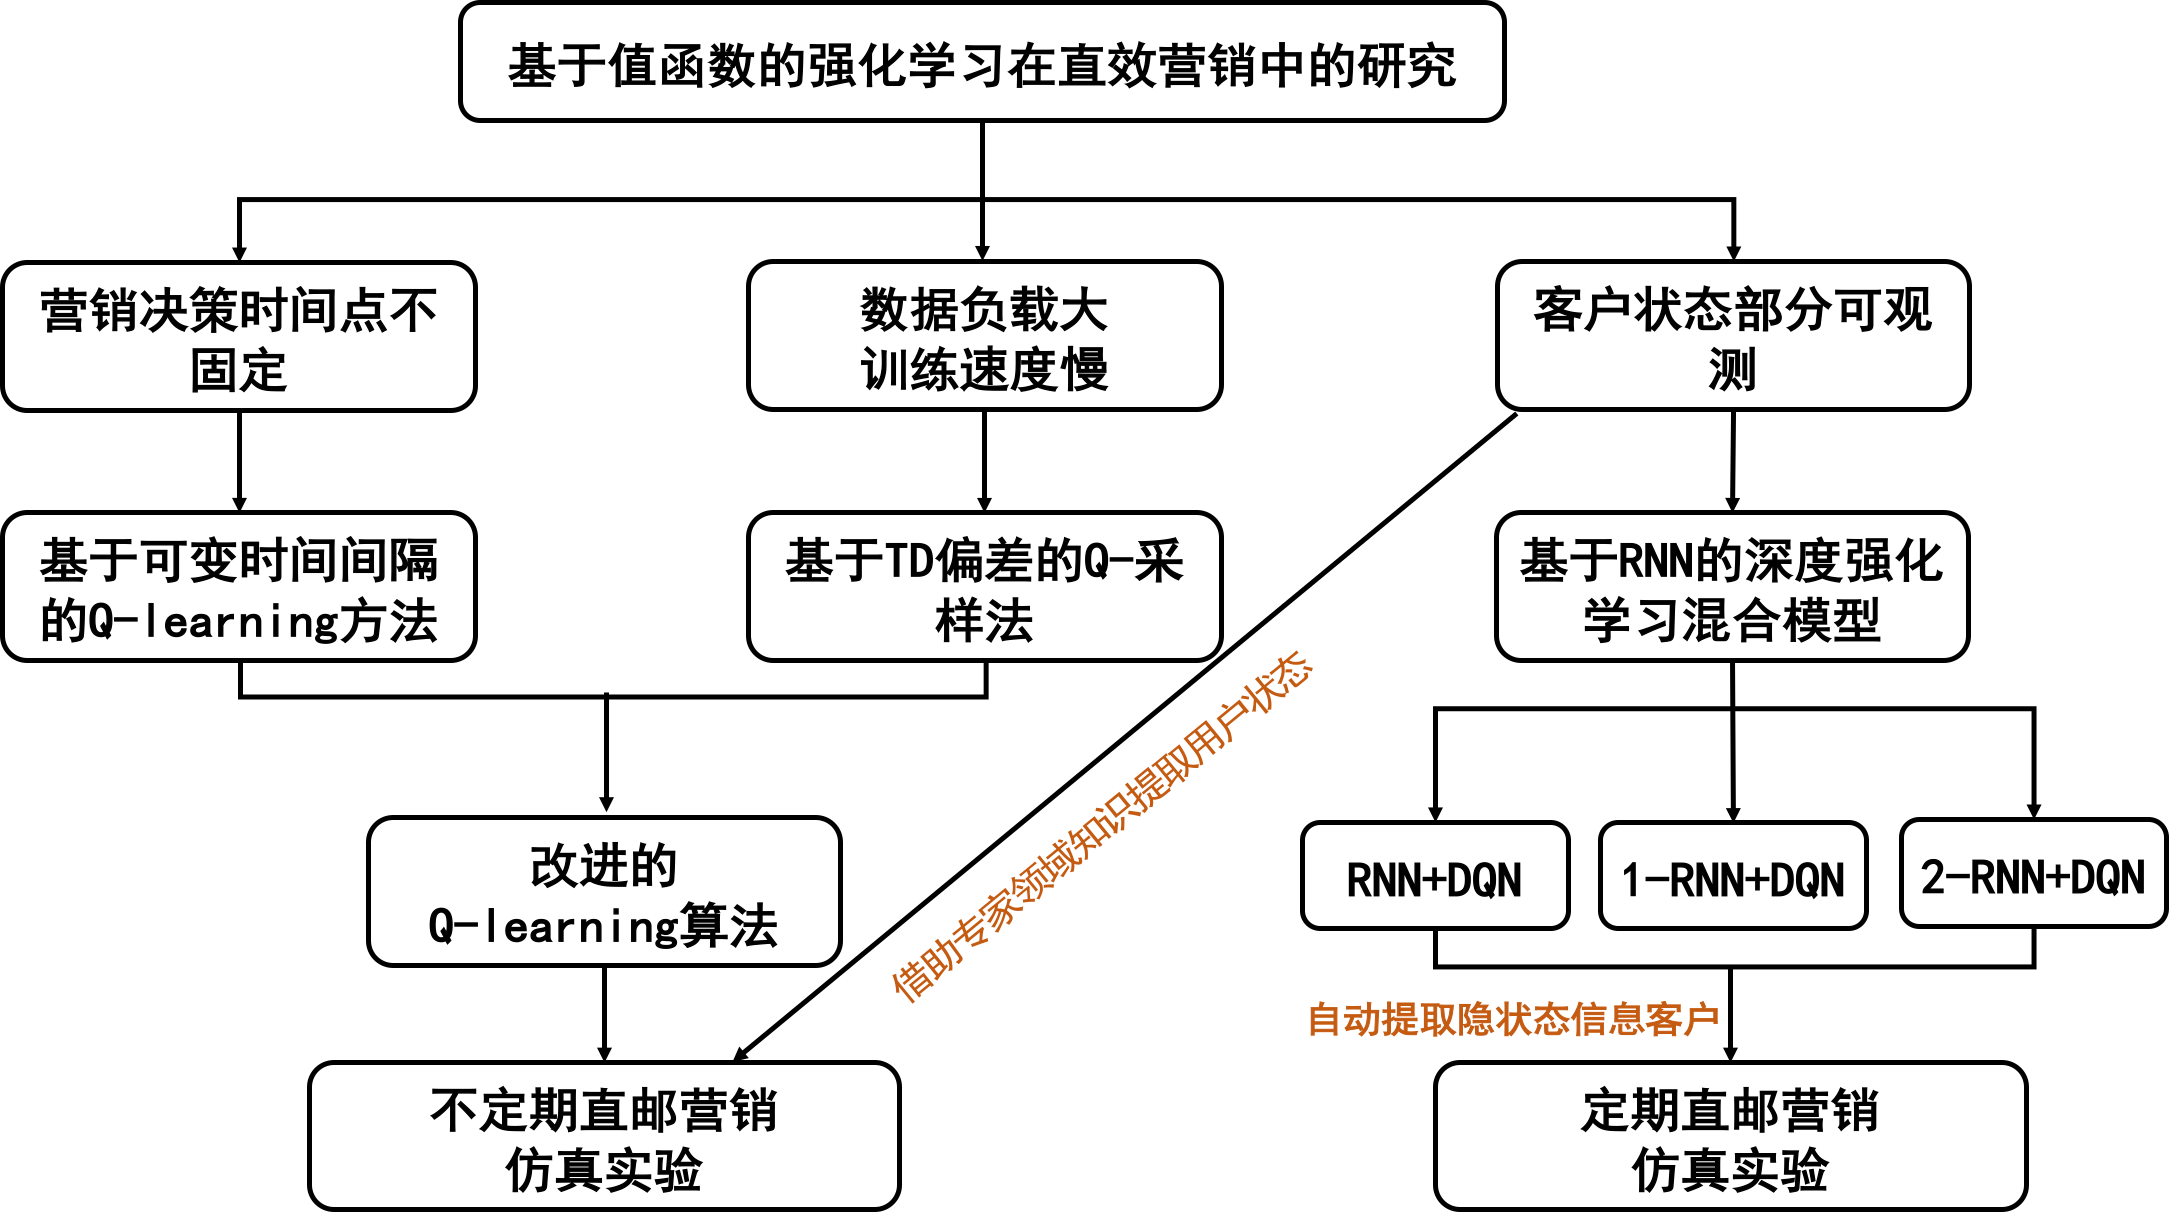
\includegraphics[width=1.0\textwidth]{研究路线图}
\caption{本文研究内容的结构图}
\label{fig:研究路线图}
\end{figure}

(1)针对直复营销场景中营销决策时间间隔不固定和数据规模大导致学习速度慢这两个问题,本文基于传统的Q-learning算法进行研究,并提出了改进的Q-learning算法。具体地,使用均值标准化的方法减少决策点间时间间隔不固定给奖赏信号带来的噪声影响,进而针对Q值函数在迭代过程中因为时间间隔更新不同步而带来的偏差,构建一个标准化因子,并仿照值函数的更新方法进行标准化因子的更新,由此提出Interval-Q算法。接着,针对Interval-Q算法在处理大规模数据时,导致训练速度慢、学习效率不高的问题,本文在Q采样法的基础上,引入TD偏差,提出基于TD偏差的Q采样法。

% 最后,通过仿真实验证明,本文所提的Interval-Q算法在不定期营销中可以取得更高的收益,另外,基于TD偏差的Q采样法,可以在减少采样数量的同时达到更好的学习效果。

(2)利用仿真环境在不定期直复营销场景中对(1)中的改进模型进行评估。
% 针对1)中的两个改进算法使用仿真环境进行评估。
其中,对于本文提出的Interval-Q算法,从策略的长期收益和策略行为的变化情况两个方面进行评估,通过实验证明Interval-Q算法因为考虑到了序列中时间间隔不固定的问题,在不定期直复营销场景中,相比传统的Q-learning算法,可以取得了更高的收益,而且具有更好的成本控制能力。接着,将本文所提出的基于TD偏差的Q采样法从长期收益和采样数两个方面与Q采样法和随机采样法进行比较,验证了所提算法在减少采样数目的同时可以取得更高的收益。需要说明的是,在以上两个实验中,为了解决客户状态的部分可观测问题,进而更好进行值函数的学习,引入了大量的专家知识来提取客户的状态信息。

(3)针对传统强化学习算法无法有效处理直复营销场景中客户状态部分可观测的问题,本文基于深度强化学习DQN模型进行研究,并提出了基于双网络的DQN模型。具体地,首先结合营销场景的时序特点,提出使用基于RNN网络的DQN模型(DQN_RNN)以学习隐状态的方式来解决上述问题。然后,通过分析指出DQN_RNN模型在网络优化过程中不能很好地同时进行隐状态的学习和值函数的逼近,由此提出基于双网络的DQN模型:通过RNN网络从监督数据中学习隐状态的表示方法,再将RNN网络输出的隐状态作为DQN网络的输入状态进行强化学习,通过这种方式可以充分发挥两个网络各自的优势,在提高值函数逼近效果的同时也能更好地学习隐状态。最后,为了取得更好的策略学习效果,又从网络结构和训练方法两个角度进行分析,提出三种改进模型:双网络独立训练模型、双网络一步联合训练模型和双网络两步联合训练模型。

(4)利用仿真环境在定期直复营销场景中对(3)中的改进模型进行评估。首先从模型的长期收益上证明本文所提出的基于双网络的DQN模型相比传统的DQN模型可以产生更多的利润,并且从三种改进模型的学习曲线和长期收益的对比中验证了本文改进方法的有效性。然后,使用不同规模的数据集对模型进行训练,实验结果表明基于双网络的DQN模型不需要利用大批量数据进行训练同样可以产生较好的营销策略。

\section{论文的结构安排}
基于监督学习和非监督学习方法在序贯决策问题中的局限性,本文考虑使用强化学习的方法来处理直复营销场景中的营销决策问题,来最大化客户的生命周期价值,进而达到最大化企业长期收益的目的。具体地,针对直复营销场景中的营销决策点时间间隔不固定和数据负载大导致训练速度慢这两个问题,在传统的Q-learning算法的基础上提出了相应的改进方案。另外,针对在实际应用中,传统的强化学习方法不能很好的处理客户状态的部分可观测问题,提出使用深度强化学习的方法以学习隐状态的方式进行解决,进一步地,为了更好的学习隐状态的表征能力,进而提高值函数的逼近效果,又提出了基于双网络的DQN模型。本文共分为五章,每章的研究内容如下:

第一章: 绪论 \quad 本章首先对直复营销的场景、目标以及本文的研究意义进行介绍,指出传统的监督学习和非监督学习在处理该问题时的局限性,并由此引出了强化学习的方法。接着,分别介绍了直复营销以及强化学习在国内外的研究现状,并结合本文的研究内容进行简要分析,指出目前研究工作中存在的的不足。最后,概括论述了本文的主要研究内容,并对论文的结构安排进行了说明。

第二章: 相关理论概述 \quad 本章首先对强化学习的学习过程进行总体阐述,以便让读者对强化学习有一个总体的认识。接着,对强化学习的理论框架以及三个基本要素(策略、回报和值函数)进行介绍。然后,针对三个基于值函数的经典的强化学习方法进行讲解,以便让读者更好地理解强化学习的思想和求解方法。最后,对值函数的逼近方法进行讨论,阐述各自的优缺点以及适应场景,特别地,对非线性函数逼近方法中DQN模型的改进点进行了详细介绍,为第四章打下理论基础。

第三章: 基于改进的Q-learning算法在不定期直复营销中的研究 \quad 本章首先介绍研究动机,即为什么要使用强化学习的方法进行直复营销策略的研究以及目前Q-learning算法在解决直复营销问题中的不足。接着,针对现实应用中存在的营销决策点间时间间隔不固定和数据负载大导致学习效率低这两个问题,结合Q-learning算法提出对应的解决方法。最后,利用数据集构建不定期直邮营销的仿真环境,对所提出的改进模型进行评估,并对仿真结果进行分析。

第四章: 基于双网络的DQN模型在定期直复营销中的研究 \quad 本章首先介绍研究动机,即为什么使用深度强化学习DQN模型来解决直复营销中的相关问题。接着,介绍DQN模型以及基于RNN的DQN模型(DQN_RNN),然后分析DQN_RNN在优化学习过程中的不足,提出了基于双网络的DQN模型,并从模型的网络结构和训练方法两个方面进行分析,提出三个改进模型:双网络独立训练模型、双网络一步联合训练模型和双网络两步联合训练模型。最后,利用数据集构建定期直邮营销的仿真环境,并对改进的模型进行评估和分析。

第五章: 总结与展望 \quad 本章系统地总结了本文的研究内容,并指出了本文工作存在的不足以及下一步的研究方向。


\cleardoublepage
% \newpage

